\section{Benchmark NIST-12 "Multiple Difficulties"}
\label{sec:bench-12}

This problem combines four aspects of benchmarks
seen in previous sections (nist-2, nist-4, nist-6 and nist-9) into one problem.
The wave front intersects the boundary
layer and corner singularity, and the peak is centered on the wave front.
The equation solved is the Poisson's equation.

\begin{equation} \label{multiple}
-\Delta u = f
\end{equation}

in the L-shaped domain, equipped with Dirichlet boundary conditions
given by the exact solution.
The exact solution:

\begin{equation}\label{exact-nist-12}
u(x,y) =  r^{\alpha_{C} }\sin(\alpha_{C} \theta) 
+ e^{-\alpha_{P} ((x - x_{P})^{2} + (y - y_{P})^{2})} 
+ tan^{-1}(\alpha_{W} (r_{W} - r_{0}))
+ e^{-(1 - y) / \epsilon}
\end{equation}

where $\alpha_C = \pi / \omega_C$, $r = \sqrt{x^2+y^2}$
and $\theta = tan^{-1}(y/x)$, here $\omega_C$ determines
the angle of the re-entrant corner.
$(x_{P}, y_{P})$ is the location of the peak, $\alpha$
determines the strength of the peak. Furthermore
$r_{W} = \sqrt{(x - x_{W})^{2} + (y - y_{W})^{2}}$,
where $(x_{W}, y_{W})$ is the center of the circular wave front,
$r_{0}$ is the distance from the wave front to the
center of the circle, and $\alpha_W$ gives
the steepness of the wave front. The parameter $\epsilon$ determines the
strength of the boundary layer, the boundary layer was placed on $y = -1$.
The right-hand side $f$ is calculated by inserting (\ref{exact-nist-12})
into (\ref{multiple}).
The solution of NIST-12 with $\omega_C = 3 \pi /2$,
$(x_{W}, y_{W}) = (0, -3/4)$, $r_{0} = 3/4$, $\alpha_{W} = 200$,
$(x_{P}, y_{P}) = (\sqrt{5} / 4, -1/4)$,
$\epsilon = 1/100$ is shown in Fig. \ref{fig:sln-nist12}.

\begin{figure}[!ht]
\centering
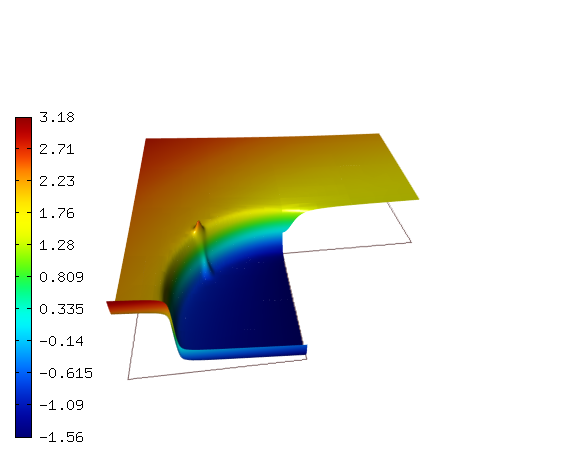
\includegraphics[height=5cm]{nist/nist-12/solution.png}
\caption{The solution to NIST-12 benchmark problem.}
\label{fig:sln-nist12}
\end{figure}

\begin{figure}[!ht]
\centering
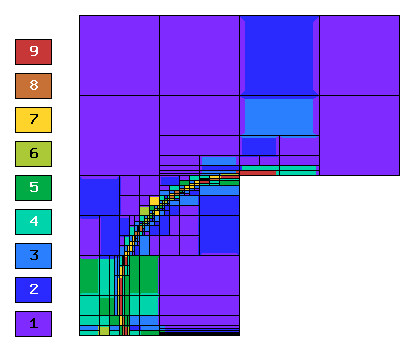
\includegraphics[height=5cm]{nist/nist-12/mesh_hp_aniso_init.png}\ \
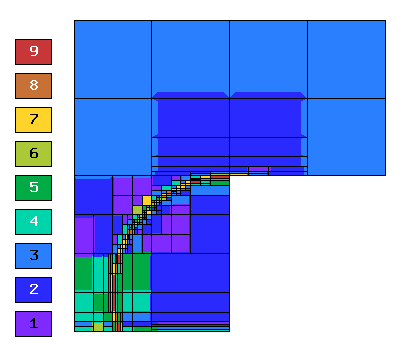
\includegraphics[height=5cm]{nist/nist-12/mesh_hp_aniso.png}
\caption{Initial mesh (left) and final mesh (right) with 4438 DOF and the resulting relative error estimate in $H^1$-norm of 9.85118e-01 \% for $hp$-FEM with anisotropic refinements.}
\label{fig:nist-12-hp-aniso}
\end{figure}

\begin{figure}[!ht]
\centering
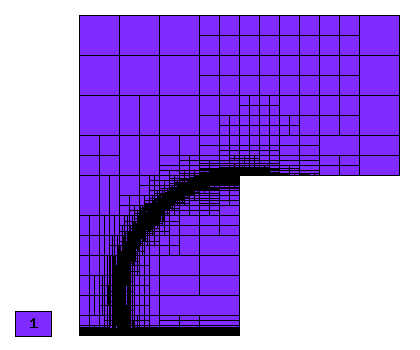
\includegraphics[height=5cm]{nist/nist-12/mesh_h1_aniso.png}\ \
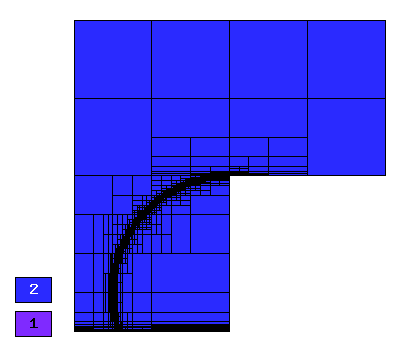
\includegraphics[height=5cm]{nist/nist-12/mesh_h2_aniso.png}
\caption{Final mesh for $h$-FEM with linear and quadratic elements.}
\label{fig:nist-12-h-aniso}
\end{figure}

Figs. \ref{fig:nist-12-conv} compare all
three approaches to automatic adaptivity from the point
of view of DOF and CPU convergence.

\begin{figure}[!ht]
\centering
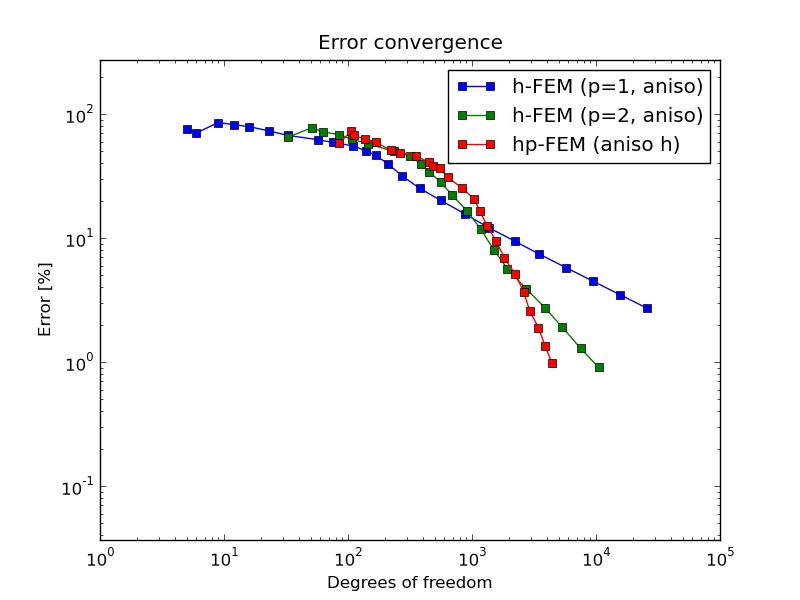
\includegraphics[height=5cm]{nist/nist-12/conv_dof_aniso.png}\ \
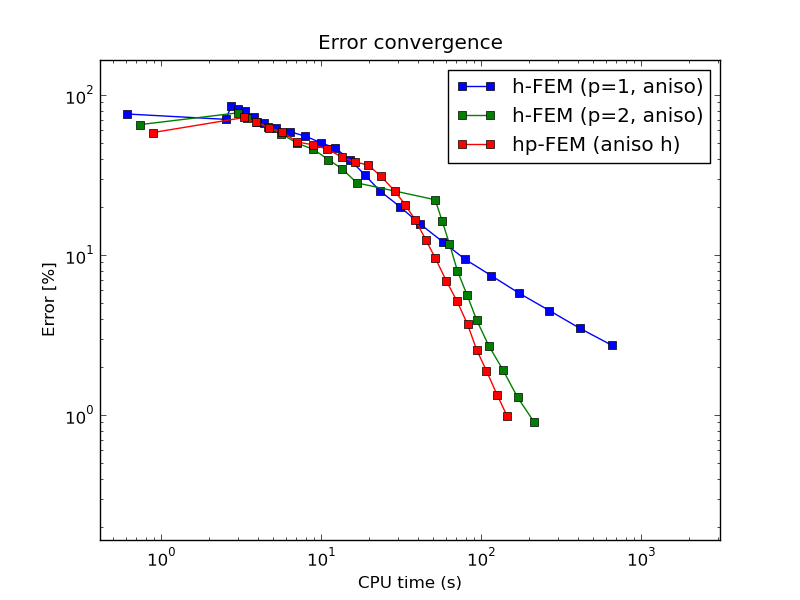
\includegraphics[height=5cm]{nist/nist-12/conv_cpu_aniso.png}
\caption{DOF and CPU time convergence graphs.}
\label{fig:nist-12-conv}
\end{figure}

